Legyen $a>1$ és
\szurkeM{
   a_{-}=\{ b\ :\ b^n < a \}\\
   a_{+}=\{ b\ :\ b^n > a \}
}
Megfigyelések:
\begin{itemize}
   \item $a_{-}$ és $a_{+}$ nemüresek
   \item bármely $b\in a_{+}$ felső korlátja $a_{-}$
   \item bármely $b\in a_{-}$ alsó korlátja $a_{+}$
\end{itemize}
A valós számok felső/alsó-határ tulajdonsága miatt egyértelműen létezik
$S=\sup a_{-}$ és $I=\inf a_{+}$ és $S\le I.$
Ha $S < I$ akkor az ábra segít megtalálni az ellentmondást:
\begin{center}
\frame{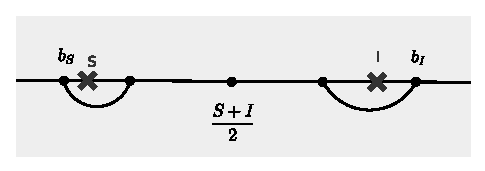
\includegraphics[scale=1.2]{DB/nthroot/fig/elso}}
\end{center}
Tehát $S=I.$ Ezért: $I^n = S^n \le a$ és $I^n\ge a$, vagyis az $S=I$ szám
valóban $a^{\frac{1}{n}}$-ként viselkedik.
%!TODO!

